
\documentclass[journal]{IEEEtran}

\ifCLASSINFOpdf
   \usepackage[pdftex]{graphicx}
  % declare the path(s) where your graphic files are
  % \graphicspath{{../pdf/}{../jpeg/}}
  % and their extensions so you won't have to specify these with
  % every instance of \includegraphics
  % \DeclareGraphicsExtensions{.pdf,.jpeg,.png}
\else
  % or other class option (dvipsone, dvipdf, if not using dvips). graphicx
  % will default to the driver specified in the system graphics.cfg if no
  % driver is specified.
   \usepackage[dvips]{graphicx}
  % declare the path(s) where your graphic files are
  % \graphicspath{{../eps/}}
  % and their extensions so you won't have to specify these with
  % every instance of \includegraphics
  % \DeclareGraphicsExtensions{.eps}
\fi

\begin{document}

\begin{figure}[t]
\begin{center}
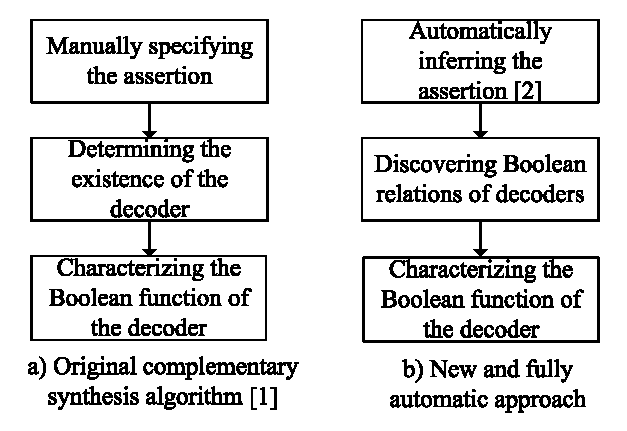
\includegraphics[width=0.35\textwidth]{flow}
\end{center}
\caption{The original and new flows of complementary synthesis}
  \label{flow}
\end{figure}


\begin{figure}[t]
\begin{center}
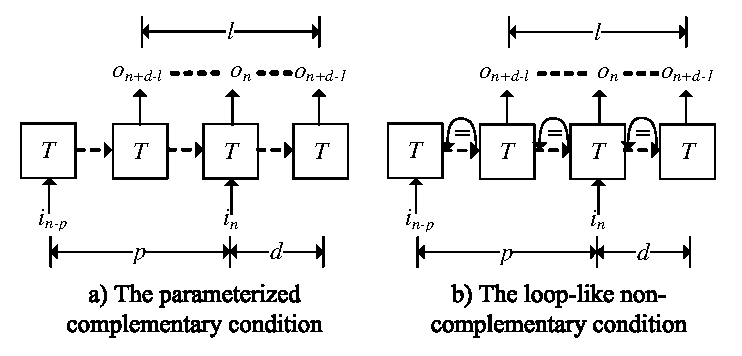
\includegraphics[width=0.5\textwidth]{pcln}
\end{center}
\caption{The parameterized complementary condition and the loop-like non-complementary condition}
  \label{fig_pcln}
\end{figure}



\begin{figure}[t]
\centering
\includegraphics[width=0.45\textwidth]{fdtest}
\caption{The SAT instance that discovers decoders}
\label{fig_fdtest}
\end{figure}

\begin{table}[t]
\centering
\caption{Information on Benchmarks}
\begin{tabular}{|c|c|c|c|c|c|}
\hline
&XGXS&XFI&scrambler&PCIE&T2 Ethernet\\\hline
\#line of verilog&214&466&24&1139&1073\\\hline
\#regs&15&135&58&22&48\\\hline
Data path width&8&64&66&10&10\\\hline
\#Config pin                              &3        &120       &1         &16      &26\\\hline
\end{tabular}\label{tab_benchmark}
\end{table}


\begin{table}[t]
\centering
\caption{Experimental Results}
\begin{tabular}{|c|c|c|c|c|c|c|}
\hline
&                                        &XG-     &XFI       &scra-     &PCI-    &T2 E-\\
&                                        &XS      &          &mbler     &E       &ther\\\hline
[10]&Runtime(sec)   &0.07    &17.84     &2.70      &0.47    &30.59\\\cline{2-7}
&$d,p,l$                                 &1,2,1   &0,3,2     &0,2,2     &2,2,1   &4,2,1         \\ \hline\hline
    &Runtime 1                           &4.53    & 264.19   &13.03     &10.39   &426.12      \\\cline{2-7}
this&Runtime 2                           &0.11    & 12.11    &1.26      &0.27    &3.07      \\\cline{2-7}
paper&Runtime 3                          &0.13    &13.69     &1.49      &0.23    &2.86      \\\cline{2-7}
    &$d,p,l$                             &1,5,1   &0,5,2     &0,5,2     &2,5,1   &4,5,1          \\ \hline %\cline{2-7}
%&\#decoders                              &1       &2         &2         &1       &1          \\ \hline
\end{tabular}\label{tab_res}
\end{table}
\end{document}


